
\documentclass{acm_proc_article-sp}
\usepackage{hyperref}

\begin{document}

\title{Linked Data-driven Web Components}
\subtitle{}

\numberofauthors{3} %  in this sample file, there are a *total*
\author{
% 1st. author
\alignauthor
Ali Khalili\\
       \affaddr{Dept. of Computer Science}\\
       \affaddr{VU University Amsterdam}\\
       \affaddr{The Netherlands}\\
       \email{a.khalili@vu.nl}
% 2nd. author
\alignauthor
Antonis Loizou\\
       \affaddr{Dept. of Computer Science}\\
       \affaddr{VU University Amsterdam}\\
       \affaddr{The Netherlands}\\
       \email{a.loizou@vu.nl}
% 3rd. author
\alignauthor
Frank van Harmelen\\
       \affaddr{Dept. of Computer Science}\\
       \affaddr{VU University Amsterdam}\\
       \affaddr{The Netherlands}\\
       \email{frank.van.harmelen@vu.nl}
}


\maketitle
\begin{abstract}
With the recent advent of Web Components, WWW is moving towards becoming a rich ecosystem of discoverable, sharable, and reusable data-driven components.
As the amount of components increase on the Web, identifying the right components and accessing the data encapsualted within these components become a challenging issue.
On the other hand, Semantic Web with the goal of understanding data on the Web has gained traction in recent years and more semantic data has become available online. 
Semantic Web and Linked Data standards provide support for richer data discovery, integration and navigation on the Web.
Linked Data-driven (LD-R) Web Components is an attempt to combine best practices for data integration from Linked Data with the development of Web components for component integration.
In this paper, we discuss the idea of semantically enhananced Web components.
In order to show the feasibility of our approach, we also present an open source software framework which enables creation and integration of LD-R Web Components.

\end{abstract}


% % A category with the (minimum) three required fields

\category{D.2.13}{Software Engineering}{Reusable Software}

\terms{Design, Human Factors, Standardization}

%\keywords{
%Linked Data, refinement operators, data cleansing, RDF transformation
%} % NOT required for Proceedings

\section{Introduction}
general about linked data applications and web components

\emph{Web Components} are a set of W3C standards that enable the creation of reusable widgets or components in Web documents and Web applications.
Web components aim to bring \emph{Component-Based Software Development} (CBSD) to the World Wide Web.
Some advantages of CBSD approach are reusibility, replacability, extensibility, encapsulation and independence.

W3C specifications of Web Components \cite{webcomponentsW3C}

introducing LD-R


Ld-R offers many benefits that we will describe in the remainder of the paper. Among them are:
-
-
\section{Contributions and Outline}
The contributions of this work are...

We evaluate this claim by...

We explore these claims in stages...


\section{Linked Data-driven Web Components}

We define a \emph{Linked Data-driven} (LD-R) Web Component as a Web component that employs RDF data model for representing its content and specification (i.e. metadata about the component).

\subsection{Features}

Linked Data-driven Web components provide the following features:

\begin{itemize}

\item \emph{Fine-grained Web applications}.
Resource Description Framework (RDF) provides a common data model that allows data-driven components to be created, shared and integrated in a structured way across different applications. \autoref{fig:architecture} depicts the 4 main component levels in a Linked Data-driven Web application.
The dataflow in the application starts from the \emph{Dataset} component which handles all the events related to a set of resources embedded in a named graph.
The next level is the \emph{Resource} component which is identified by a URI and indicates what is described in the application.
A resource is specified by a set of properties which are handled by the \emph{Property} component. Properties can be either individual or aggregate when combining multiple features of a resource (e.g. a component that combines longitude and latitude properties; start datae and end date properties for a date range, etc.).
Each property is instantiated by an individual value or mutiple values in case of an aggreagte object. 
The value(s) of properties are controled by the \emph{Object} component.
Object component invokes different components to view, edit and browse the property values.
\emph{Viewer}, \emph{Editor} and \emph{Browser} components are terminals in the LD-R single directional data flow where customized user-generated components can be plugged into the system.
These components apply on individual and aggregate objects (e.g. to show multiple coordinates on a the map).

\begin{figure}[tb]
  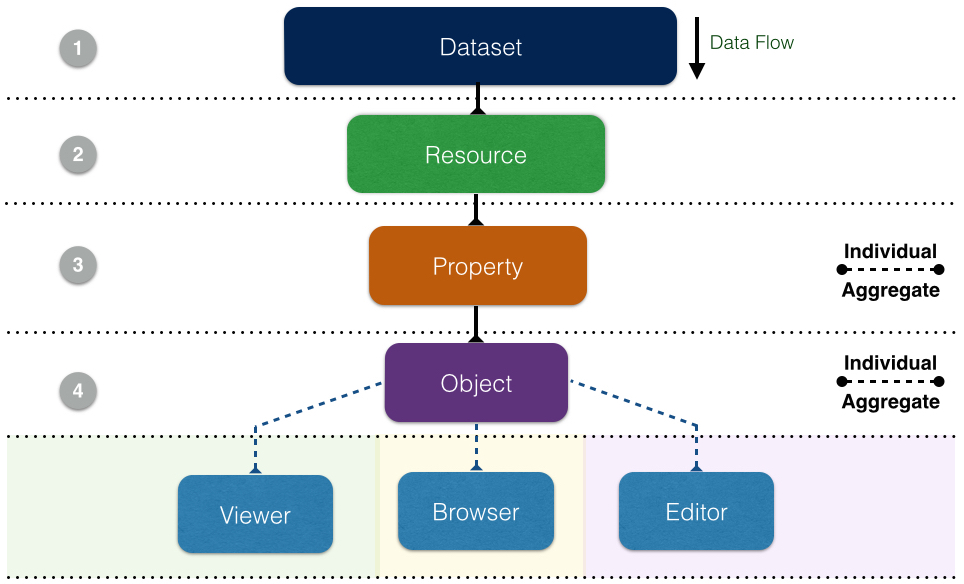
\includegraphics[width=.9\linewidth]{images/architecture.jpg}
  \caption{Architecture of LD-R Applications.}
  \label{fig:architecture}
\end{figure}

In addition to the fine-grained component architecture, LD-R Web applications provide a fine-grained access control over the data provided by the components.
RDF-based access control in LD-R applications operates at four different granularities provided by Dataset, Resource, Property and Object component levels.
For example, we can restrict access to a specific property of a specific resource in a certain dataset.

\begin{figure}[tb]
  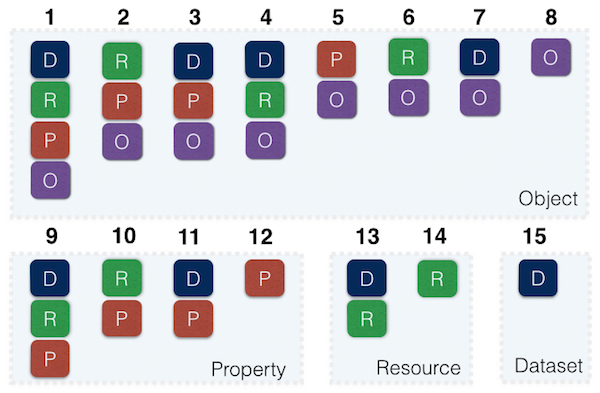
\includegraphics[width=.9\linewidth]{images/scopes.jpg}
  \caption{LD-R Scopes.}
  \label{fig:scopes}
\end{figure}

\item \emph{Customization and Personalization}.
LD-R provide a versatile approach for context adaptation.
A context can be a specific domain of interest, a specific user requirments or both.
In order to enable customization and personalization, LD-R exploits the concept of \emph{Scope}.
A scope is defiened as a directed combination of Dataset, Resource, Property and Object components (cf. \autoref{fig:scopes}).
Each scope conveys a certain level of specificity on a given context ranging from 1 (most specific) to 15 (least specfic).
Scopes are defined by using the URIs for RDF resources and types.
For example, on the property level, we can define a generic configuration for all properties and then for some specific properties (e.g. dcterms:title, rdfs:label) within a specific resource (e.g. <http://ld-r.org>), we can change or overwrite those configurations.

Scopes can also be defined under a specific user which facilitates versioning and reuse of user-specific configs.
User-specifc configs provide different views on components and thereby data, based on the different personas dealing with those components and data.

\item \emph{Component Visibility and Reusability}.

metadata about components (https://github.com/ali1k/ld-r-metadata-generator) in JSON-LD

general metadata: name, description, version, homepage, author, etc.

specific metadata: level, granularity (individual, aggregate), mode (view, edit, browse), dependencies (internal, external), config parameters with description

use Schema.org SoftwareApplication schema.

\item \emph{Content Visibility and Reusability}.

Component content represented in RDFa, Microdata. exmaple: good relations for online shopping and SEO



\end{itemize}



\subsection{Life Cycle}

\begin{figure}[tb]
  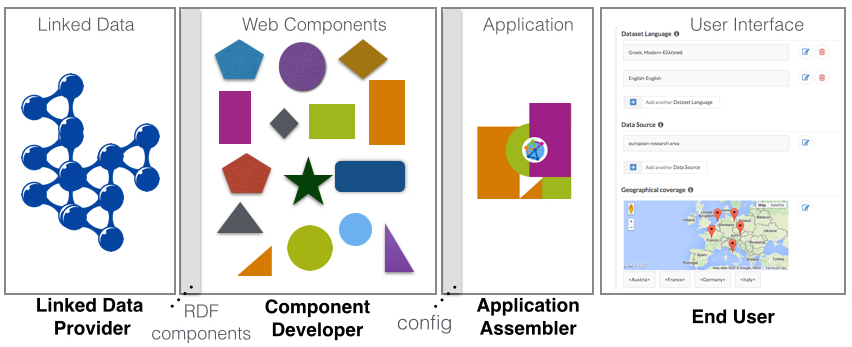
\includegraphics[width=1\linewidth]{images/lifecycle.jpg}
  \caption{LD-R Components Life Cycle.}
  \label{fig:lifecycle}
\end{figure}

As shown in \autoref{fig:lifecycle}, the LD-R components lifecycle encompasses four primary types of stakeholders:

\begin{itemize}

\item \emph{Linked Data Provider}.
Since the LD-R approach focuses mainly on Linked Data applications, provision of RDF-compliant data is an essential phase in developing the LD-R components.
*Data Scientists and different steps in providing fata from LOD2 project

\item \emph{Component Developer}. 
It includes programmers who are involved in component fabrication.


\item \emph{Application Assembler}.
The main task of application assembler is to identify the right components and configurations for the application; and combine them in a way which fits the application requirement. 

\item \emph{End User}. 
It is the user who experiences working with components to pursue his goals on a certain application domain.
The end user is the one who requests developing a component and the one who sends feedback on the existing components.

\end{itemize}

\section{Implementation}

In order to realize the idea of Linked Data-driven Web components, we implemented a software framework called \emph{Linked Data Reactor (LD-R)} which is available online at \url{http://ld-r.org}.
LD-R utilizes Facebook's ReactJS\footnote{\url{https://facebook.github.io/react/}} components and Flux\footnote{\url{https://facebook.github.io/flux}} architecture, Yahoo!'s Fluxible\footnote{\url{http://fluxible.io/}} framework for isomorphic Web applications and Semantic-UI\footnote{\url{http://semantic-ui.com/}} framework for flexible UI themes.


\begin{figure}[tb]
  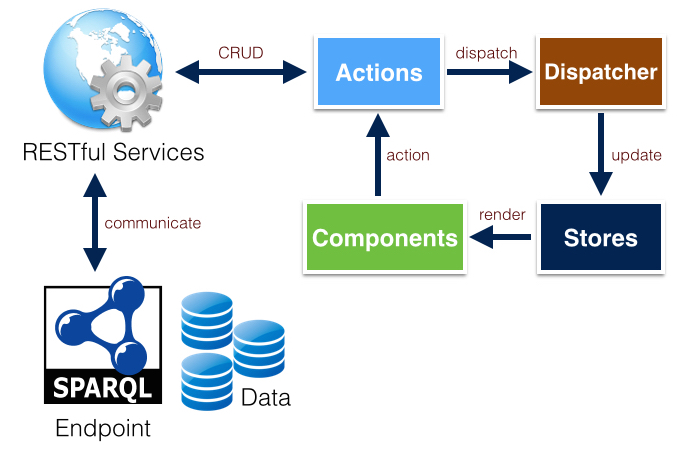
\includegraphics[width=.9\linewidth]{images/dataflow.jpg}
  \caption{Data Flow in LD-R framework.}
  \label{fig:dataflow}
\end{figure}

The main reasons we chose \emph{React} components over other existing solutions (e.g. Polymer\footnote{\url{http://www.polymer-project.org/}}, AngularJS\footnote{\url{https://angularjs.org/}}, EmberJS\footnote{\url{http://emberjs.com/}}, etc.) were the maturity of the technology, maintainablity, number of developer tools/components/applications, and efficiency\footnote{Elaborating on all these factors is beyond the scope of this paper.}.
As shown in \autoref{fig:dataflow}, LD-R follows the Flux architecture which eschews MVC (Model-View-Controller) in favor of a unidirectional data flow. 
When a user interacts with a React component, the component propagates an action through a central dispatcher, to the various stores that hold the application's data and business logic, which updates all of the components that are affected. 
The component interaction with SPARQL endpoints to retrieve and update Linked Data occurs via invoking RESTful services in actions.

\begin{figure}[tb]
  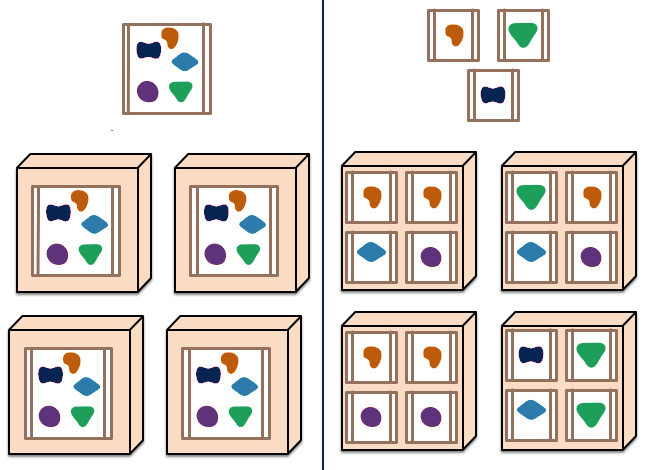
\includegraphics[width=.9\linewidth]{images/microservices.jpg}
  \caption{Monoliths vs. Microservices~\cite{microservices}}
  \label{fig:microservices}
\end{figure}

In contrast to the centalized monolithic architecture, LD-R applications comply with \emph{Microservices Architecture}~\cite{microservices}.
Microservices architecture puts each element of component functionality into a separete service and scales by distributing these services across servers, replicating as needed.


\begin{figure}[tb]
  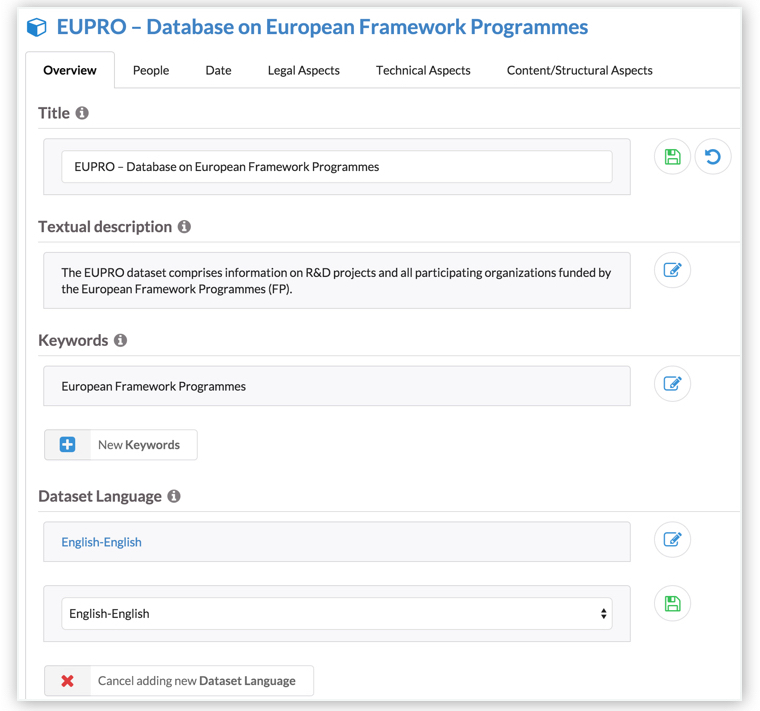
\includegraphics[width=.9\linewidth]{images/screenshot.jpg}
  \caption{Screenshot}
\end{figure}

\section{Evaluation}

RISIS

OpenPhacts

\section{Discussion}

\section{Related Work}

Web Components and the Semantic Web~\cite{pahl2011}

Semantic Web Services

Existing tools to view/edit and browse LD e.g. OntoWiki, Saha

\section{Conclusion}

LD-R approach not only facilitates the discovery and reuse of Web components but also makes the creation of Linked Data application easier.

\section{Aknowledgement}
We would like to thank our colleagues from the KRR research group at VU University Amsterdam for their helpful comments during the development of the LD-R framework. This work was supported by a grant from the European Union's 7th Framework Programme provided for the project RISIS (GA no. 313082).


\bibliographystyle{abbrv}
\bibliography{refs}

\end{document}
